\title{Networking and System Security \\ Assignment 2}
\author{David van Erkelens (10264019) \\ Department of Computer Science \\ University of Amsterdam}
\date{\today}
\documentclass[12pt]{article}
\usepackage{graphicx}
\usepackage{xcolor}
\begin{document}
\maketitle
\section{Task 1}
\begin{enumerate}
	\item The IP address of the executing host is \verb|192.168.2.10|, and the IP address of the target host is \verb|192.16.191.44|
	\item The source host sends only one packet every time.
	\item The executing hosts sends a couple of packets with a short time to live, and then receives a returning ICMP value: this can be 11 (\verb|Time-to-live exceeded|), which means the target host is not reached yet, or code 0 (\verb|Echo (ping) reply|). Each time code 11 is received, the IP address of the last visited note is returned and a packet with a longer time to live is send. During this process, all intermediate nodes are traced.
	\item The destination node is 15 hops away.
	\item The IP address of the executing host is \verb|192.168.2.10|, and the IP address of the target host is \verb|147.102.222.213|
	\item UDP traceroute works almost the same als ICMP traceroute. The only difference is that with UDP traceroute, not only the time to live increments, but also the destination port. It is not sure if the destination accepts traffic on this port; we simply hope for an ICMP code 3 - \verb|Port unreacable|, which would mean the destination is reached.
	\item The destination node is 19 hops away.
\end{enumerate}
\section{Task 2}
\begin{enumerate}
	\setcounter{enumi}{7}
	\item 
	\begin{itemize}
		\item \verb|www.mit.edu| - {\color{red} Unavailable}
		\item \verb|www.facebook.com| - {\color{green} Available}
		\item \verb|www.cwi.nl| - {\color{green} Available}
		\item \verb|www.ntua.gr| - {\color{green} Available}
		\item \verb|www.twitter.com| - {\color{green} Available}
	\end{itemize}
	Some sites may not respond because their firewall might not accept ICMP packets - this could possibly be to protect their sites from the bad guys trying to overload their sites or something similair. 
	\item The last responding node is \verb|OC11-RTR-1-BACKBONE-2.MIT.EDU (18.168.1.41)|
	\item
	\begin{itemize}
		\item \verb|www.facebook.com| - 17 ms
		\item \verb|www.cwi.nl| - 9 ms
		\item \verb|www.ntua.gr| - 72 ms
	\end{itemize}
	This difference can be simply explained: the distance between the client and the server is bigger for foreign hosts than domestic or worldwide hosts. Just a rule of nature.
	\item Twitter:
	\begin{verbatim}
 		5  ge-3-3-0.mpr1.ams1.nl.above.net (64.125.25.13)  1.192 ms 
 		6  so-2-0-0.mpr1.lhr3.uk.above.net (64.125.30.129)  8.514 ms 
 		7  xe-4-3-0.cr2.dca2.us.above.net (64.125.24.41)  82.132 ms 
	\end{verbatim}
	MIT:
	\begin{verbatim}
 		5  ae-56-221.ebr2.Amsterdam1.Level3.net (4.69.153.201)  0.816 ms 
 		6  ae-48-48.ebr2.London1.Level3.net (4.69.143.82)  8.188 ms 
 		7  ae-43-43.ebr1.NewYork1.Level3.net (4.69.137.74)  76.996 ms 
	\end{verbatim}
	This can be simply explained: this is where the package goes international en crosses a huge distance: so the response takes a little more time to reach the client.
	\item Ping results (in Dutch, with edited commands for Windows):
	\begin{verbatim}
	C:\Users\David>ping -n 10 -l 24 www.cwi.nl

Pingen naar www.cwi.nl [192.16.191.44] met 24 bytes aan gegevens:
Antwoord van 192.16.191.44: bytes=24 tijd=12 ms TTL=56
Antwoord van 192.16.191.44: bytes=24 tijd=8 ms TTL=56
Antwoord van 192.16.191.44: bytes=24 tijd=8 ms TTL=56
Antwoord van 192.16.191.44: bytes=24 tijd=7 ms TTL=56
Antwoord van 192.16.191.44: bytes=24 tijd=9 ms TTL=56
Antwoord van 192.16.191.44: bytes=24 tijd=9 ms TTL=56
Antwoord van 192.16.191.44: bytes=24 tijd=9 ms TTL=56
Antwoord van 192.16.191.44: bytes=24 tijd=10 ms TTL=56
Antwoord van 192.16.191.44: bytes=24 tijd=9 ms TTL=56
Antwoord van 192.16.191.44: bytes=24 tijd=10 ms TTL=56

Ping-statistieken voor 192.16.191.44:
    Pakketten: verzonden = 10, ontvangen = 10, verloren = 0
    (0% verlies).

De gemiddelde tijd voor het uitvoeren van één bewerking in milliseconden:
    Minimum = 7ms, Maximum = 12ms, Gemiddelde = 9ms

C:\Users\David>ping -n 10 -l 8000 www.cwi.nl

Pingen naar www.cwi.nl [192.16.191.44] met 8000 bytes aan gegevens:
Antwoord van 192.16.191.44: bytes=8000 tijd=16 ms TTL=56
Antwoord van 192.16.191.44: bytes=8000 tijd=16 ms TTL=56
Antwoord van 192.16.191.44: bytes=8000 tijd=16 ms TTL=56
Antwoord van 192.16.191.44: bytes=8000 tijd=15 ms TTL=56
Antwoord van 192.16.191.44: bytes=8000 tijd=15 ms TTL=56
Antwoord van 192.16.191.44: bytes=8000 tijd=15 ms TTL=56
Antwoord van 192.16.191.44: bytes=8000 tijd=17 ms TTL=56
Antwoord van 192.16.191.44: bytes=8000 tijd=18 ms TTL=56
Antwoord van 192.16.191.44: bytes=8000 tijd=16 ms TTL=56
Antwoord van 192.16.191.44: bytes=8000 tijd=26 ms TTL=56

Ping-statistieken voor 192.16.191.44:
    Pakketten: verzonden = 10, ontvangen = 10, verloren = 0
    (0% verlies).

De gemiddelde tijd voor het uitvoeren van één bewerking in milliseconden:
    Minimum = 15ms, Maximum = 26ms, Gemiddelde = 17ms
	\end{verbatim}
	This higher delay can be explained by the fact that the transmission delay is bigger for large packages.
\end{enumerate}
\section{Task 3}
\begin{enumerate}
	\setcounter{enumi}{12}
	\item \verb|Switch.ch:| \\
	\textbf{Number of routes:} 10 \\
	\textbf{Average delay:} 28 ms\\ \\
	\verb|Ntua.gr:| \\
	\textbf{Number of routes:} 12\\
	\textbf{Average delay:} 51 ms\\ \\
	\item The last four nodes are the same:
	\begin{verbatim}
		surfnet-gw.rt1.ams.nl.geant.net (62.40.124.158) 
		AE2.500.JNR01.Asd001A.surf.net (145.145.80.78) 
		V1131.sw4.amsterdam1.surf.net (145.145.19.170)
		www.surfnet.nl (145.0.2.10) 
	\end{verbatim}
	\item Also here, the biggest delays are introduced when the packages travel larger distances.
	\clearpage
	\item During the making of this assignment, the Australian server reported an server error, so this assignment could not be made. \\ \\
	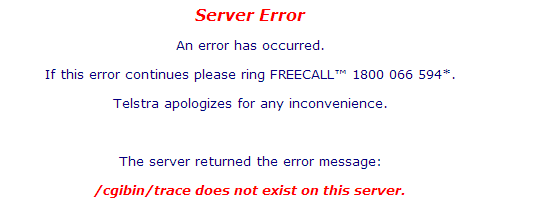
\includegraphics{error.png}
	\item There are multiple routers in one single link. For example:
	\begin{verbatim}
		12  ae2.bb01.iad2.tfbnw.net (204.15.20.88)  90.6 ms (ttl=242!)  
		    ae2.bb02.iad2.tfbnw.net (74.119.77.148)  85.5 ms (ttl=242!)
	\end{verbatim}
	This could be explained by the fact that there are multiple router routes between the client and \verb|Facebook.com|, or like we Dutch people would say: "Er zijn meerdere wegen naar Rome" - meaning there are multiple paths to travel to your final destination.
\end{enumerate}
\end {document}